\documentclass[48pt]{article}
\usepackage{CJK}
\usepackage{listings}
\usepackage{xcolor}
\usepackage[margin=1in]{geometry}
\usepackage{amsmath,amsthm,amssymb}
\usepackage{graphicx}
\usepackage{epstopdf}
\DeclareGraphicsExtensions{.eps,.ps,.jpg,.bmp}
\lstset{
	numbers=left,
    framexleftmargin=10mm,
    frame=none,
    backgroundcolor=\color[RGB]{245,245,244},
	keywordstyle=\bf\color{blue},
	identifierstyle=\bf,
	numberstyle=\color[RGB]{0,192,192},
	commentstyle=\it\color[RGB]{0,96,96},
	stringstyle=\rmfamily\slshape\color[RGB]{128,0,0},
	showstringspaces=false
    }

\newcommand{\N}{\mathbb{N}}
\newcommand{\R}{\mathbb{R}}
\newcommand{\Z}{\mathbb{Z}}
\newcommand{\Q}{\mathbb{Q}}

\newenvironment{theorem}[2][Theorem]{\begin{trivlist}
\item[\hskip \labelsep {\bfseries #1}\hskip \labelsep {\bfseries #2.}]}{\end{trivlist}}
\newenvironment{lemma}[2][Lemma]{\begin{trivlist}
\item[\hskip \labelsep {\bfseries #1}\hskip \labelsep {\bfseries #2.}]}{\end{trivlist}}
\newenvironment{exercise}[2][Exercise]{\begin{trivlist}
\item[\hskip \labelsep {\bfseries #1}\hskip \labelsep {\bfseries #2.}]}{\end{trivlist}}
\newenvironment{problem}[2][Problem]{\begin{trivlist}
\item[\hskip \labelsep {\bfseries #1}\hskip \labelsep {\bfseries #2.}]}{\end{trivlist}}
\newenvironment{question}[2][Question]{\begin{trivlist}
\item[\hskip \labelsep {\bfseries #1}\hskip \labelsep {\bfseries #2.}]}{\end{trivlist}}
\newenvironment{corollary}[2][Corollary]{\begin{trivlist}
\item[\hskip \labelsep {\bfseries #1}\hskip \labelsep {\bfseries #2.}]}{\end{trivlist}}

\begin{document}

\title{Homework 2016-03-11}
\author{Chuan Lu\\
13300180056}

\maketitle

\begin{problem}{1}
\text{ }\\
Display the Runge Phenomenon.
\end{problem}

\begin{proof}
\subsection{The code is shown as follows.}
\begin{lstlisting}[language={MATLAB}]
function [ value ] = newton_coefficient( given_points, function_values )
    n = length(function_values);
    for i =1: n - 1
    	function_values(i+1:n) = (function_values(i+1:n) - function_values(i:n - 1))
    		./ (given_points(i+1:n) - given_points(1:n - i));
%             disp(f_values(i:n));
    end
    value = function_values;
    
\end{lstlisting}

\begin{lstlisting}[language={MATLAB}]
function [ f_series ]  = Newton_eval( given_points, function_values, eval_points)
%NEWTON_EVAL  
args = newton_coefficient( given_points, function_values );

f_series = polynomail_eval(args, eval_points, given_points);

% plot( eval_points, f_series );
\end{lstlisting}

\begin{lstlisting}[language = {MATLAB}]
function [value] = polynomail_eval( args, eval_points, given_points )
value = args( length( args ) );
for i = length( args ) - 1:-1:1
    value = value .* (eval_points - given_points( i ) )
     + args( i );
end;
\end{lstlisting}

\begin{lstlisting}[language = {MATLAB}]
f = @(x)(1 ./ (1 + 25 * (x .^ 2)));
plot_points = -1:1e-6:1;
yy = feval(f, plot_points);
plot(plot_points, yy);
hold on

for n = 4:4:12
    given_points = -1:1/n:1;
    function_values = feval(f, given_points);
    f_series = Newton_eval(given_points, function_values, plot_points);
    plot(plot_points, f_series);
    hold on
end
axis([-1, 1, -1, 1]);
legend('f(x)', 'n = 4', 'n = 8', 'n = 12', 'Location', 'best');
\end{lstlisting}

\subsection{The result is shown as follows.}
\begin{figure}[htbp]
\centering
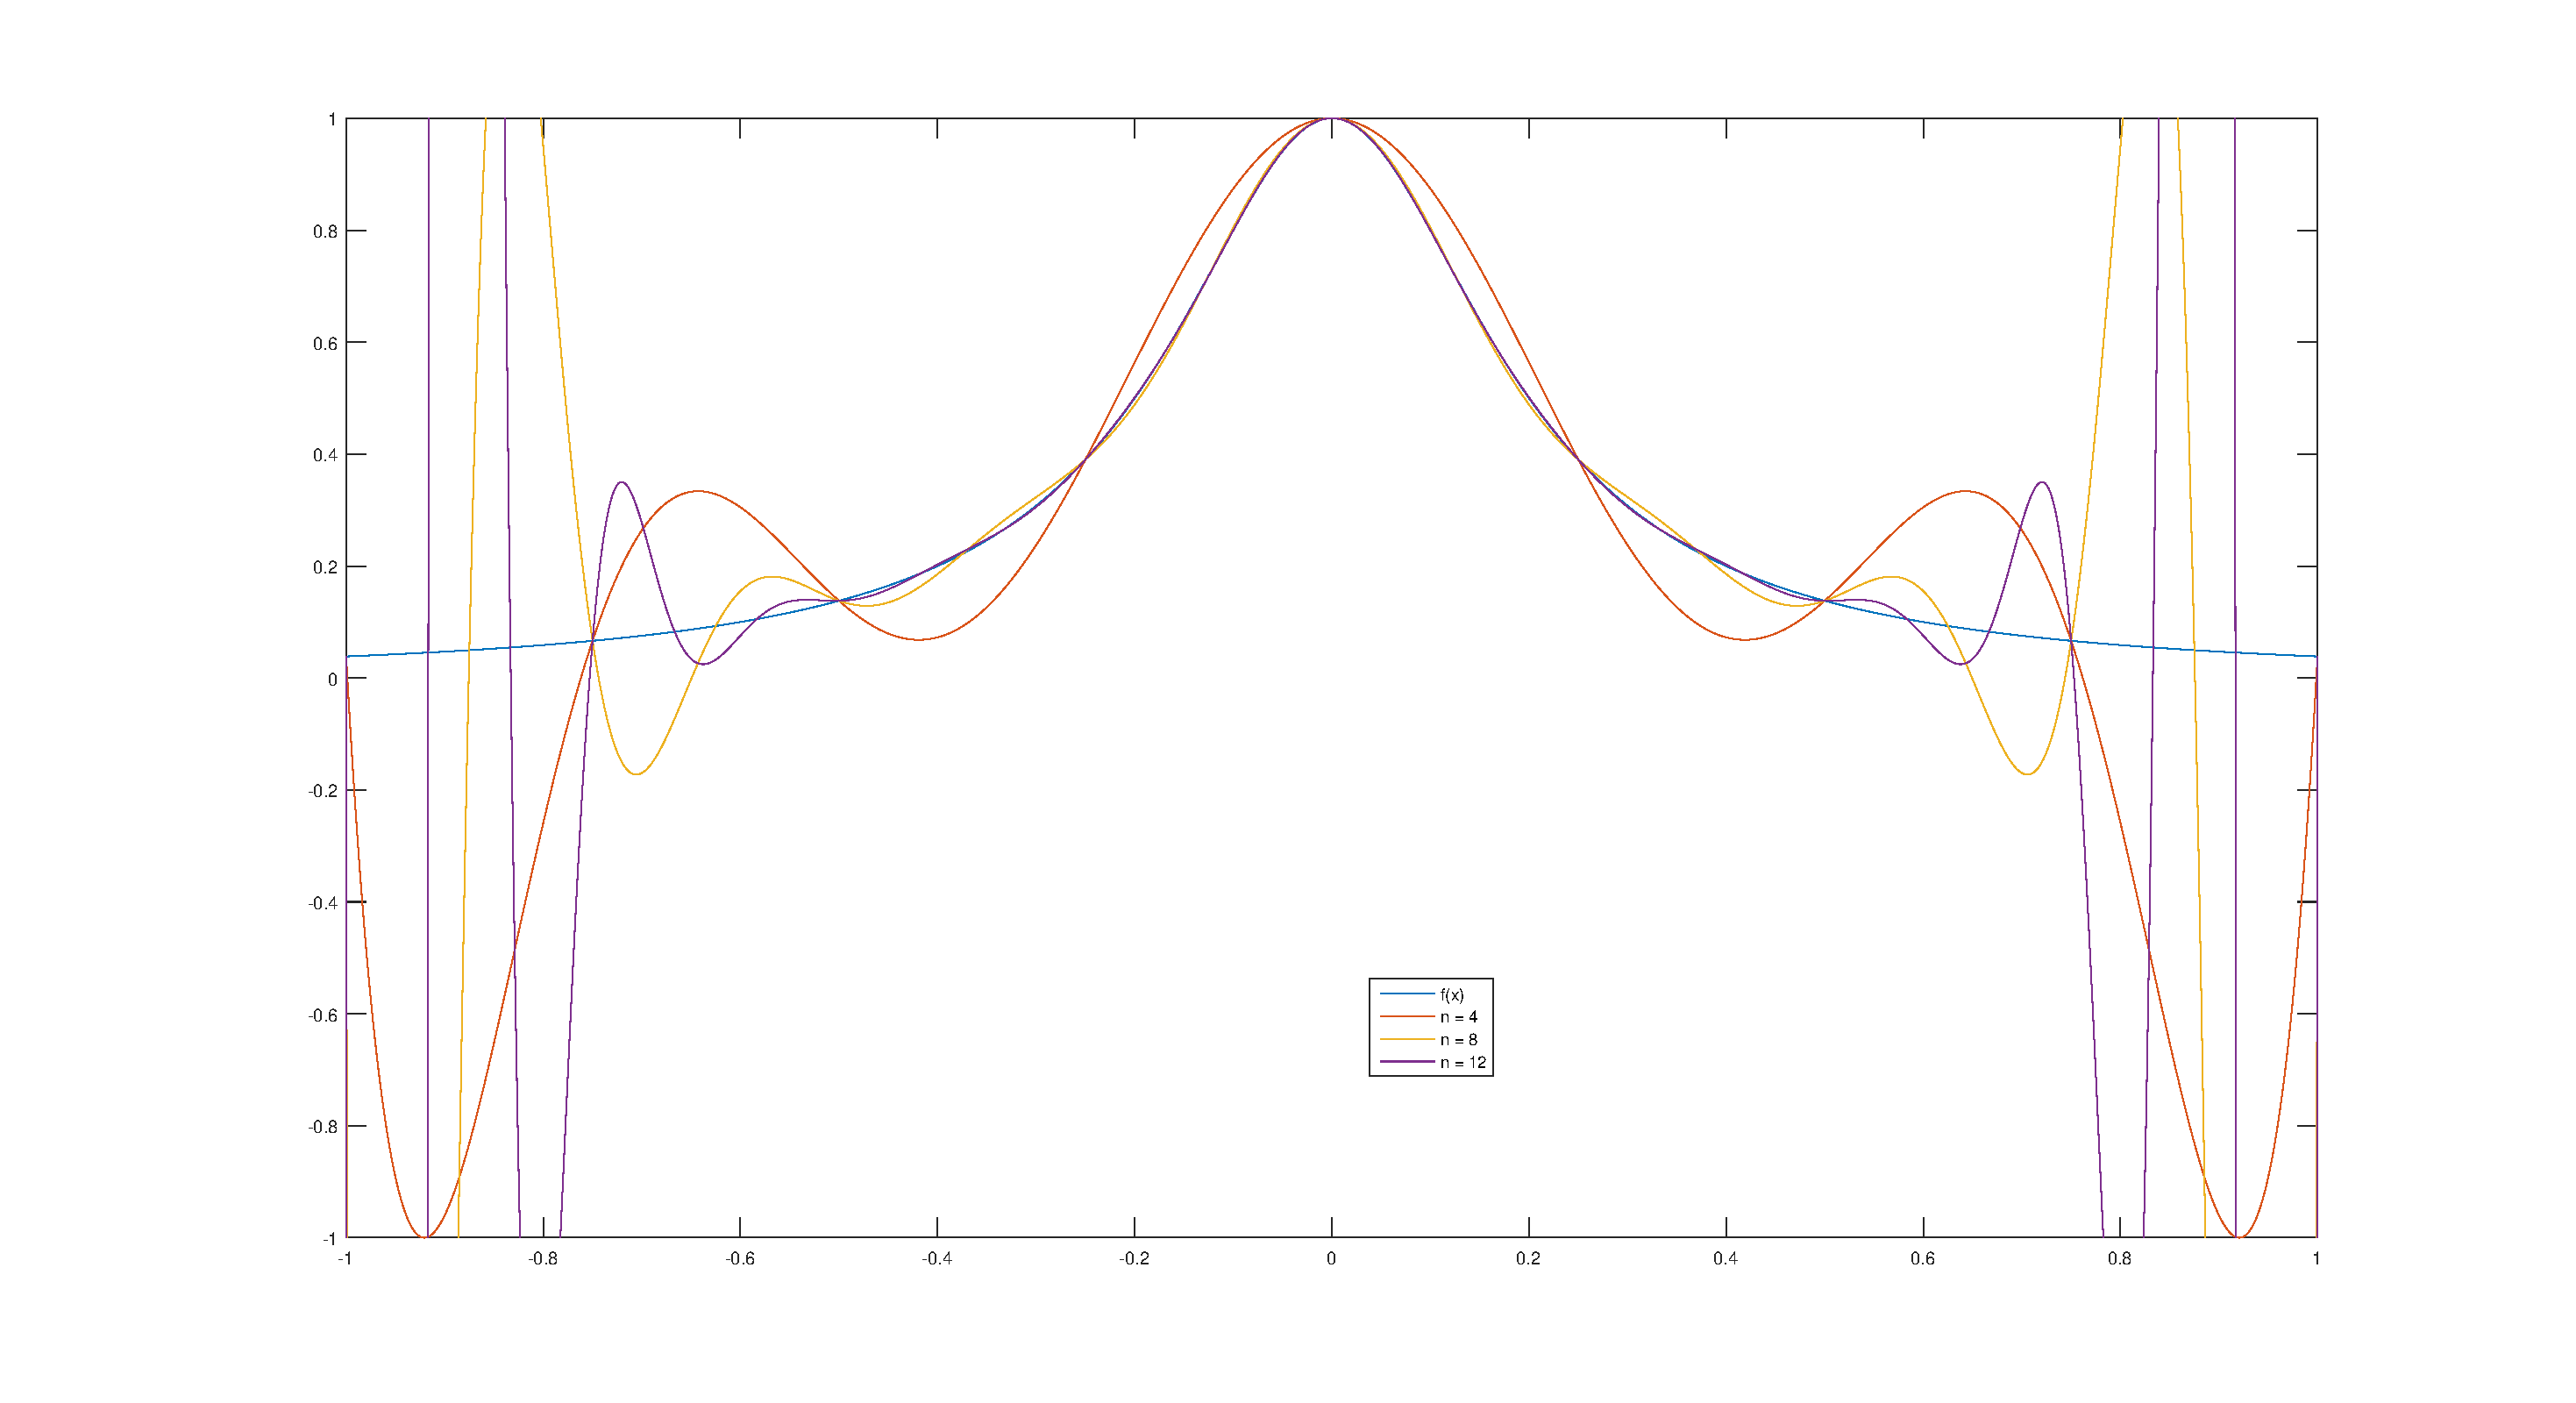
\includegraphics[width = 15cm]{runge.eps}
\caption{The Runge Phenomenon}
\label{Runge}
\end{figure}
\end{proof}

\begin{problem}{2}
\text{ }\\
Calculate the integral of $x^{n}$ with Newton-Cotes Formula.
\end{problem}
\begin{proof}
\subsection{The code is shown as follows.}

\begin{lstlisting}[language = {MATLAB}]
function [ coeff ] = cotes_coefficient( order )
%Calculate the cotes coefficient with the order given
%Use the equation given at Page179, exercise3
n = order
matrix = zeros(n, n);
for i = 1 : n
    matrix( i , : ) = (1:n) .^ i;
end
c = (n .^ (1:n)) ./ (2:n+1);
c = transpose(c);
coeff = matrix \ c;
coeff = [coeff(n); coeff];
end
\end{lstlisting}

\begin{lstlisting}[language = {MATLAB}]
function[ coeff ] = get_coeff( order )
% get_coeff of newton_cotes formula of interval
% order means the order of the formula
switch order
    case 1
        coeff = [1, 1];
    case 2
        coeff = [1, 4, 1];
    case 3
        coeff  = [1,3,3,1];
    case 4
        coeff = [7,32, 12, 32, 7];
    case 5
        coeff = [19, 75, 50, 50, 75, 19];
    case 6
        coeff = [41, 216, 27, 272, 27, 216, 41];
    case 7
        coeff = [751, 3577, 1323, 2989, 2989, 1323, 3577, 751];
    case 8
        coeff = [989, 5888, -928, 10496, -4540, 10496, -928, 5888, 989];
    otherwise
        error('order should be between 0 and 8 --get_cotes_coeff');
end
    coeff = coeff / sum(coeff);
\end{lstlisting}

\begin{lstlisting}[language = {MATLAB}]
function [ coeff ] = new_cotes_coefficient( order )
%Calculate the cotes coefficient with the order given
%Use the equation given at Page179, exercise3
n = order;
matrix = zeros(n, n);
for i = 1 : n
    matrix( i , : ) = (((1:n) ./ n) .^ i);
end
c = 1 ./ ( 2: n + 1);
c = transpose(c);
coeff = matrix \ c;
coeff = [coeff(n); coeff];
end
\end{lstlisting}

\begin{lstlisting}[language = {MATLAB}]
function [ result ] = newton_cotes( func, inteval, order )
%NEWTON_COTES Use Newton_Cotes Formula to Calculate the intergral.

if nargin < 2
    error(' Too few inputted arguments, please check if function and inteval for integrating have been inputted or not  -- Newton_Cotes');
elseif nargin == 2
    order = 2;
end

if order < 0 || order > 8
    error(' Order Error: The order should be between 0 and 8. --Newton_Cotes ');
end

low = inteval( 1 );
high = inteval( 2 );

if order == 0
    result = feval(func, (low + high) / 2) * (high - low);
else
    coeff = get_coeff(order);
    eval_points = low : (high - low) / order : high;
    eval_points = transpose( eval_points );
    result = sum( coeff * feval(func, eval_points)) * (high - low);
end
\end{lstlisting}

\begin{lstlisting}[language = {MATLAB}]
function func = get_func( n )
    func = @(x)(x .^ n);
\end{lstlisting}

\begin{lstlisting}[language = {MATLAB}]
% Homework1.3.1
inteval = [0, 1];
result_matrix = zeros(7, 6);
for n = 1:7
    func = get_func(n);
    result_matrix(n, 1) = integral(func, 0, 1);
    for order = 0:4
        func = get_func(n);
        result_matrix(n, order + 2) = newton_cotes(func, inteval, order);
    end
end
disp(result_matrix)
\end{lstlisting}

\subsection{The result is shown as the table above.}

\begin{table}
\begin{tabular}{c|c|c|c|c|c|c}
    \hline
    & Exact Value & medium formula & trapezium formula & Simpson formula & 3/8 formula & Cotes formula \\
    \hline
    $x^{1}$ & 0.5000 & 0.5000 & 0.5000 & 0.5000 & 0.5000 & 0.5000 \\
    \hline
    $x^{2}$   & 0.3333  &  0.2500  &  0.5000 &  0.3333  &  0.3333  &  0.3333 \\
    \hline
    $x^{3}$ & 0.2500  &  0.1250 &   0.5000 & 0.2500  &  0.2500    &    0.2500 \\
    \hline
    $x^{4}$  & 0.2000 &   0.0625  &  0.5000  & 0.2083 &   0.2037    &   0.2000 \\
    \hline
    $x^{5}$   &  0.1667  &  0.0313 &  1 0.5000 &   0.1875 &  0.1759  &  0.1667 \\
    \hline
    $x^{6}$  &   0.1429  &  0.0156  &  0.5000  &  0.1771  &  0.1584  &  0.1432 \\
    \hline
    $x^{7}$   &  0.1250  &  0.0078  &  0.5000  &  0.1719   & 0.1471  &  0.1263 \\
    \hline
    \end{tabular}
    \caption{Integral of $x^{n}$ using Newton-Cotes Formula}
    \end{table}
\end{proof}
\end{document}
\begin{lstlisting}[language={MATLAB}]
% make matrix
% author: chuanlu
% 2016-03-02
function [A] = make_matrix(op, n)

    if nargin < 1
        error('More args needed --make matrix');
    elseif nargin == 1
        op = 'A1';
    end

    if op == 'A1'
        c1 = zeros(1, n - 1);
        c1(2 : n - 1) = -3;
        c2 = zeros(1, n - 2) + 2;
        A = eye(n) + diag(c1, -1) + diag(c2, -2);
    elseif op == 'A2'
        c1 = zeros(1, n - 1);
        c1(2 : n - 1) = -3;
        c2 = zeros(1, n - 2) + 2;
        A = eye(n) + diag(c1, -1) + diag(c2, -2);
        A(1, n) = -1;
    else
        error('Operation Failed to Match A1 or A2');
    end
\end{lstlisting}

% \begin{lstlisting}[language={MATLAB}]
% % homework2.m
% % author: chuanlu
% % 2016-03-02

% op1 = 'A1';
% op2 = 'A2';
% N = 100;
% cond1 = zeros(1, N);
% cond2 = zeros(1, N);
% for n = 1 : N
%     A1 = make_matrix(op1, n);
%     A2 = make_matrix(op2, n);
%     cond1(n) = cond(A1);
%     cond2(n) = cond(A2);
% end
% n = [1:N];
% figure(1);
% semilogy(n, cond1, '*-');
% figure(2);
% plot(n, cond2, '*-');
% %     disp('cond1:');
% %     disp(cond1);
% %     disp('cond2:');
% %     disp(cond2);
% \end{lstlisting}
% The result is shown as follows.
% \end{proof}

% \begin{problem}{3}
% \text{ }\\
% Given $\Vert x_{n+2} - x_{n+1} \Vert$  $\leqslant$ $\alpha\Vert x_{n+1} - x_{n} \Vert$, then $\Vert x^{\star} - x_{n} \Vert$ $\leqslant$ $\frac{\alpha_{n}}{1-\alpha}\Vert x_{1} - x_{0}\Vert$.
% \end{problem}

% \begin{proof}
% $\Vert x_{n} - x_{n - 1} \Vert\leqslant\alpha\Vert x_{n - 1} - x_{n - 2} \Vert\leqslant\dots\leqslant\alpha^{n-1}\Vert x_{1} - x_{0}\Vert$ \\
% \par Hence, $\Vert x_{\star} - x_{n} \Vert\leqslant\Vert x_{n} - x_{n+1} \Vert+\Vert x_{n+1} - x_{n+2}\Vert + \dots\leqslant(\alpha^{n}+\alpha^{n+1}+\dots)\Vert x_{1} - x_{0}\Vert$ \\
% \par$= \frac{\alpha^{n}}{1-\alpha}\Vert x_{1} - x_{0}\Vert$
% \end{proof}

\end{document}
% % \begin{problem}{4}
% % \text{ }\\
% % Suppose that $[a]$ is a unit in $\Z_{n}$ and $[b]$ is an element of $\Z_{n}$. Prove that the equation $[a]x = b$ has exactly one solution in $\Z_{n}$
% % \end{problem}

% % \begin{proof}

% % \end{proof}

% % \begin{problem}{5}
% % \text{ }\\
% % Suppose that $[a]$ and $[b]$ are both units in $\Z_{n}$.  Show that the product $[a] \cdot [b]$ is also a unit in $\Z_{n}.$ (Note that this confirms closure under multiplication in the group $U_{n})$.
% % \end{problem}

% % \begin{proof}

% % \end{proof}

% % \begin{problem}{6}
% % \text{ }\\
% % Which of the following are Groups? Which of the following are not groups, and why?\\

% % \indent (1)  $G = \{{2, 4, 6, 8}\}$ in $\Z_{10}$.  Where $a \star b = ab$\\
% % \indent (2)  $G = \Q^{\ast}$, where $a \star b = \frac{a}{b}$\\
% % \indent (3) $G = \Z$, where $a \star b = a - b$\\
% % \indent (4) $G = \{ {2^{x}\mid x \in \Q} \}$, where $a \star b = ab$\\

% % \end{problem}

% % \begin{proof}

% % \end{proof}

% % \begin{problem}{7}
% % \text{ }\\
% % Consider the set $Q =$ \{ $\pm$1, $\pm$i, $\pm$j, $\pm$k\} of the complex matrices as follows:\\
% % \[
% % 1=
% %   \begin{bmatrix}
% %     1 & 0\\
% %     0 & 1\\
% %   \end{bmatrix}
% % \]

% % \[
% % i=
% %   \begin{bmatrix}
% %     i & 0\\
% %     0 & $-$i\\
% %   \end{bmatrix}
% % \]

% % \[
% % j=
% %   \begin{bmatrix}
% %     0 & 1\\
% %     $-$1 & 0\\
% %   \end{bmatrix}
% % \]

% % \[
% % k=
% %   \begin{bmatrix}
% %     0 & i\\
% %     i & 0\\
% %   \end{bmatrix}
% % \]
% % Show that $Q$ is a group under matrix multiplication by writing out its multiplicaiton table. (Note: $Q$ is called the quartenion group).
% % \end{problem}
% % \begin{proof}

% % \end{proof}

% % \end{document}
